\documentclass[a4paper,14pt]{extarticle}

\usepackage[a4paper,top=20mm,bottom=20mm,left=30mm,right=10mm]{geometry}
\usepackage[T1,T2A]{fontenc}
\usepackage[utf8]{inputenc}
\usepackage[russian]{babel}
\usepackage{indentfirst}
\usepackage{titlesec}
\usepackage{graphicx}
\usepackage{verbatim}
\usepackage{fancyvrb}
\usepackage{nicematrix}
\usepackage{hyperref}

\renewcommand{\baselinestretch}{1.3}

\titleformat{\section}{\normalsize\bfseries}{\thesection}{1em}{}
\titleformat{\subsection}{\normalsize\bfseries}{\thesubsection}{1em}{}

\setlength{\parindent}{12.5mm}

\begin{document}

  \newpage\thispagestyle{empty}
  \begin{center}
    \MakeUppercase{
      Министерство науки и высшего образования Российской Федерации\\
      Федеральное государственное бюджетное образовательное учреждение высшего образования\\
      <<Вятский Государственный Университет>>\\
    }
    Институт математики и информационных систем\\
    Факультет автоматики и вычислительной техники\\
    Кафедра электронных вычислительных машин
  \end{center}
  \vfill

  \begin{center}
    Отчет по лабораторной работе №5\\
    по дисциплине\\
    <<Информатика>>\\
    <<Сборки без программирования>>\\
    Вариант 9
  \end{center}
  \vfill

  \noindent
  \begin{tabular}{ll}
    Выполнил студент гр. ИВТб-1301-05-00 \hspace{5mm} & \rule[-1mm]{25mm}{0.10mm}\,/Макаров С.А./ \\
    Руководитель преподаватель & \rule[-1mm]{25mm}{0.10mm}\,/Шмакова Н.А./ \\
  \end{tabular}

  \vfill
  \begin{center}
    Киров 2025
  \end{center}

  \newpage
  \section*{\hspace{12.5mm}Цель работы}
  Цель работы: Закрепление основ работы с Arduino.

  \section*{\hspace{12.5mm}Задание}
  \begin{enumerate}
    \item Игра на реакцию
    \item Секретный код. Секретный код должен соответствовать номеру варианта.
    \item Дешифратор. Без Arduino, без программирования. Только с использованием изученных микросхем и микросхем стандартной логики. Для отображения результата можно использовать светодиоды.
    \item Секундомер на два семисегментных индикатора. Без Arduino, без программирования. Только с использованием изученных микросхем и микросхем стандартной логики.
  \end{enumerate}

  \newpage
  \section*{\hspace{12.5mm}Решение}
  \subsection*{\hspace{12.5mm}Задание 1}
  Выполнена живая сборка.

  \subsection*{\hspace{12.5mm}Задание 2}
  Выполнена живая сборка. \\

  \noindent Таблица 1 -- Таблица истинности\\
  \begin{NiceTabular}{ccccc}[hvlines, cell-space-top-limit=1mm]
    $x_3$ $x_2$ $x_1$ $x_0$ & $x_3$ $\overline{x_2}$ $\overline{x_1}$ $x_0$ & $x_3 x_2$ $x_1$ $x_0$ & $x_3 x_2 x_1$ $x_0$ & $x_3 x_2 x_1 x_0$\\

    0 0 0 0 & 0 1 1 0 & 0 1 0 & 0 0 & 0 \\
    0 0 0 1 & 0 1 1 1 & 0 1 1 & 0 1 & 0 \\
    0 0 1 0 & 0 1 0 0 & 0 0 0 & 0 0 & 0 \\
    0 0 1 1 & 0 1 0 1 & 0 0 1 & 0 1 & 0 \\
    0 1 0 0 & 0 0 1 0 & 0 1 0 & 0 0 & 0 \\
    0 1 0 1 & 0 0 1 1 & 0 1 1 & 0 1 & 0 \\
    0 1 1 0 & 0 0 0 0 & 0 0 0 & 0 0 & 0 \\
    0 1 1 1 & 0 0 0 1 & 0 0 1 & 0 1 & 0 \\
    1 0 0 0 & 1 1 1 0 & 1 1 0 & 1 0 & 0 \\
    1 0 0 1 & 1 1 1 1 & 1 1 1 & 1 1 & 1 \\
    1 0 1 0 & 1 1 0 0 & 1 0 0 & 0 0 & 0 \\
    1 0 1 1 & 1 1 0 1 & 1 0 1 & 0 1 & 0 \\
    1 1 0 0 & 1 0 1 0 & 0 1 0 & 0 0 & 0 \\
    1 1 0 1 & 1 0 1 1 & 0 1 1 & 0 1 & 0 \\
    1 1 1 0 & 1 0 0 0 & 0 0 0 & 0 0 & 0 \\
    1 1 1 1 & 1 0 0 1 & 0 0 1 & 0 1 & 0 \\
  \end{NiceTabular}\\

  \subsection*{\hspace{12.5mm}Задание 3}
  Схема сборки программы предаставлена на рисунке 1, принципиальные схемы предаставлены на рисунках 2, 3. Проект в Tinkerkad: \href{https://www.tinkercad.com/things/e4K54R4CD0k-lr-5-3-deshifrator/editel?returnTo=%2Fdashboard%2Fdesigns%2Fcircuits&sharecode=-Hv8qgPniVeXdUa-nYDvK8NiAmY0oiQlfKNoSDOx3QA}{ссылка на рабочий проект}. \\

  \noindent Таблица 2 -- Таблица истинности\\
  \begin{NiceTabular}{cccc}[hvlines, cell-space-top-limit=1mm]
    Двоичное & Код Грея & +9 & \\
    $x_1$ $x_2$ $x_3$ $x_4$ & $x_1$ $x_2$ $x_3$ $x_4$ & $x_1$ $x_2$ $x_3$ $x_4$ & ($1 \oplus x_4 \land x_1 \oplus 1$) $x_4$ $x_3$ $x_2$ $x_1$ $x_0$  \\

    0 0 0 0 & 0 0 0 0 & 1 0 0 1 & 0 1 0 0 1 \\
    0 0 0 1 & 0 0 0 1 & 1 0 1 0 & 0 1 0 1 0 \\
    0 0 1 0 & 0 0 1 1 & 1 1 0 0 & 0 1 1 0 0 \\
    0 0 1 1 & 0 0 1 0 & 1 0 1 1 & 0 1 0 1 1 \\
    0 1 0 0 & 0 1 1 0 & 1 1 1 1 & 0 1 1 1 1 \\
    0 1 0 1 & 0 1 1 1 & 0 0 0 0 & 1 0 0 0 0 \\
    0 1 1 0 & 0 1 0 1 & 1 1 1 0 & 0 1 1 1 0 \\
    0 1 1 1 & 0 1 0 0 & 1 1 0 1 & 1 0 1 0 1 \\
    1 0 0 0 & 1 1 0 0 & 0 1 0 1 & 1 0 1 1 0 \\
    1 0 0 1 & 1 1 0 1 & 0 1 1 0 & 1 1 0 0 0 \\
    1 0 1 0 & 1 1 1 1 & 1 0 0 0 & 1 0 1 1 1 \\
    1 0 1 1 & 1 1 1 0 & 0 1 1 1 & 1 0 0 1 1 \\
    1 1 0 0 & 1 0 1 0 & 0 0 1 1 & 1 0 1 0 0 \\
    1 1 0 1 & 1 0 1 1 & 0 1 0 0 & 1 0 1 0 0 \\
    1 1 1 0 & 1 0 0 1 & 0 0 1 0 & 1 0 0 1 0 \\
    1 1 1 1 & 1 0 0 0 & 0 0 0 1 & 1 0 0 0 1 \\
  \end{NiceTabular}\\

  \begin{figure}[h]
    \centering
    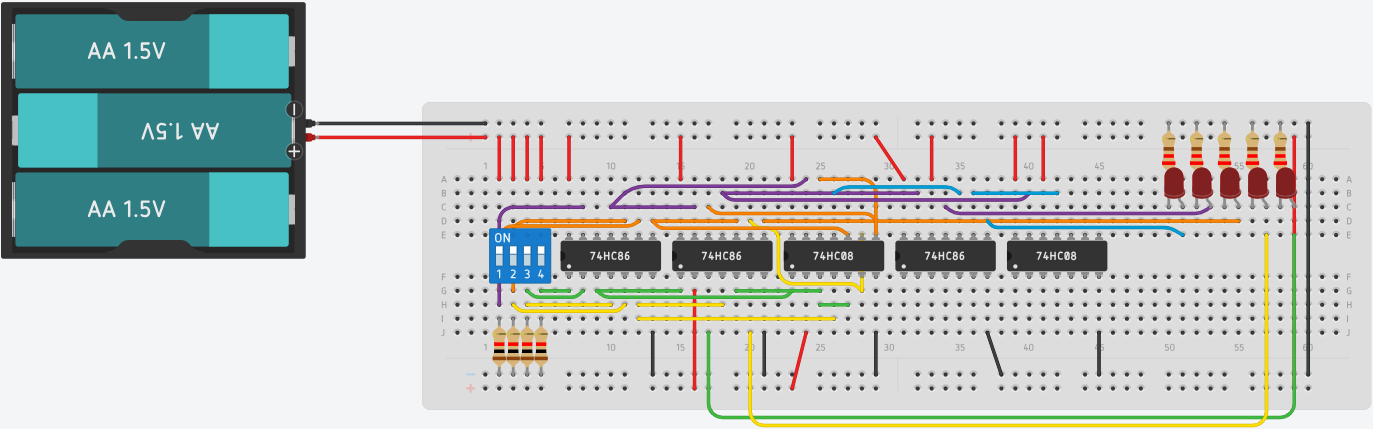
\includegraphics[width=1\linewidth]{images/image-1}
  \end{figure}
  \begin{center}
    Рисунок 1 – Схема сборки на макетной плате
  \end{center}

  \pagebreak

  \begin{figure}[h]
    \centering
    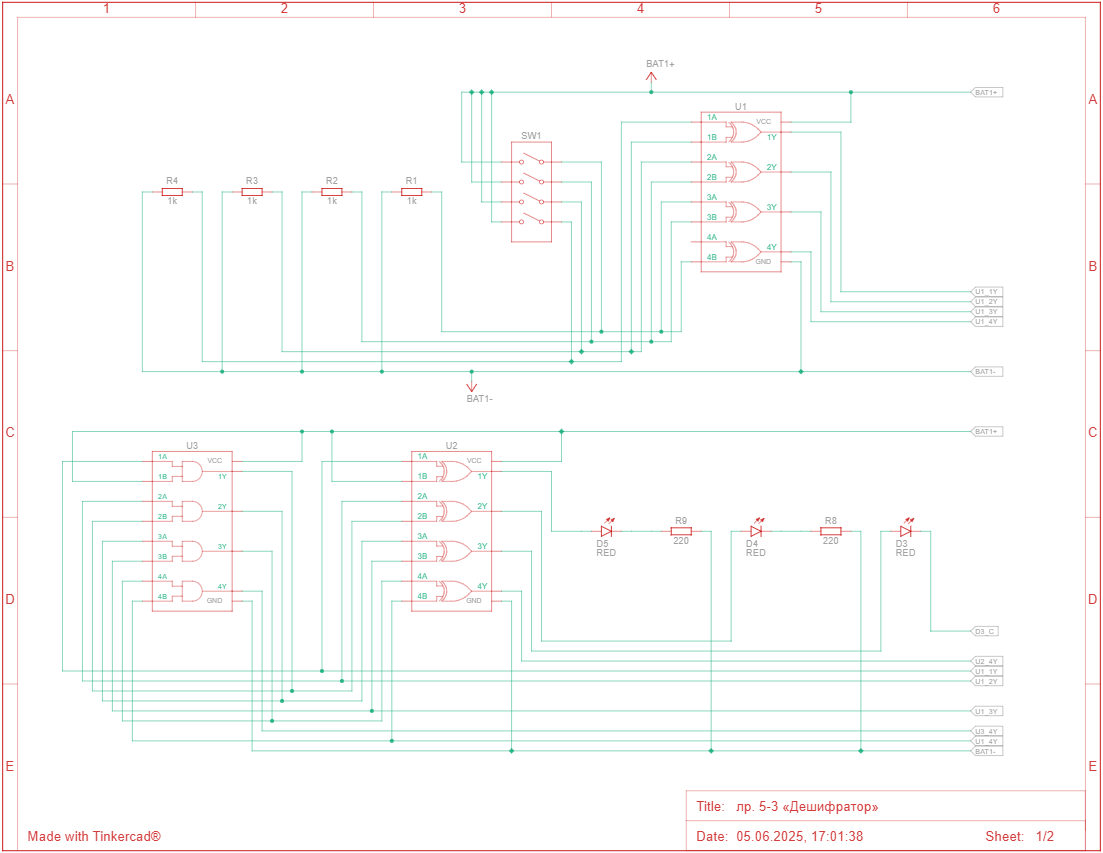
\includegraphics[width=0.72\linewidth]{images/image-2}
  \end{figure}
  \begin{center}
    Рисунок 2 – Принципиальная схема
  \end{center}

  \begin{figure}[h]
    \centering
    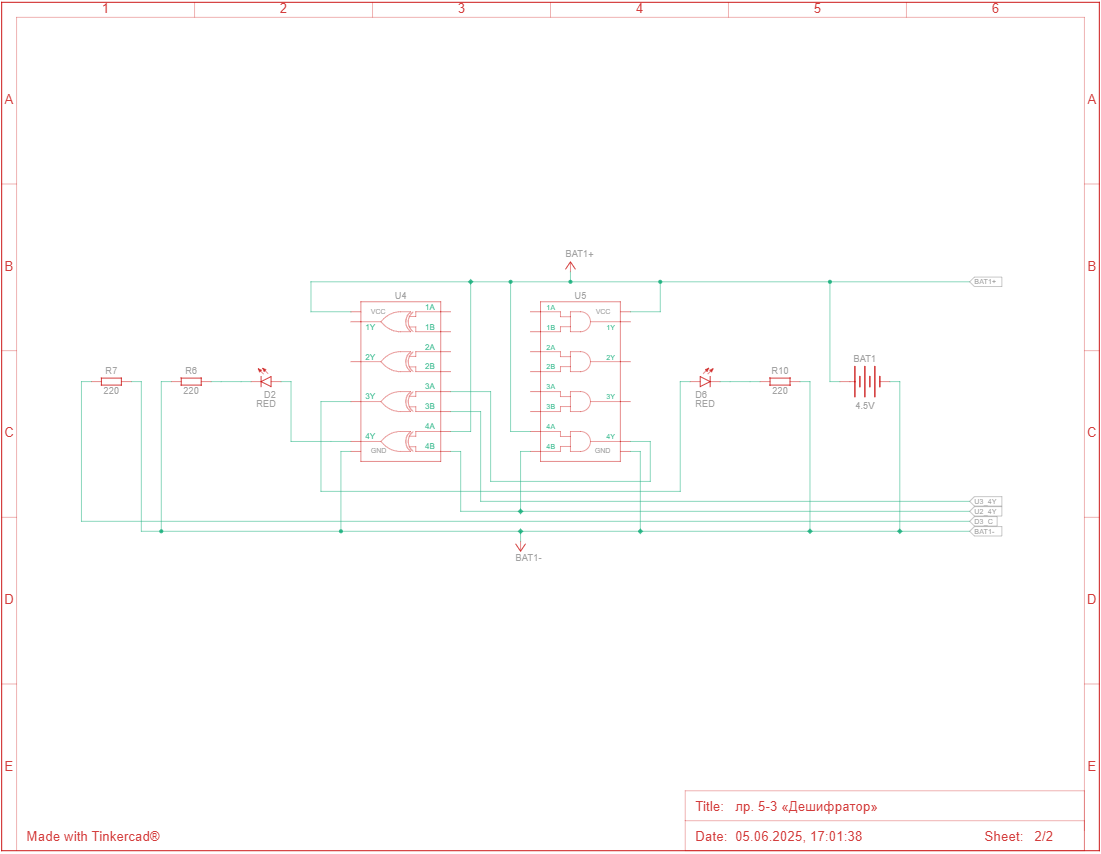
\includegraphics[width=0.72\linewidth]{images/image-3}
  \end{figure}
  \begin{center}
    Рисунок 3 – Принципиальная схема
  \end{center}

  \subsection*{\hspace{12.5mm}Задание 4}
  Схема сборки программы предаставлена на рисунке 4, принципиальные схемы предаставлены на рисунках 5, 6. Проект в Tinkerkad: \href{https://www.tinkercad.com/things/9LRhfF1oQmo-lr-5-4-sekundomer-svoj/editel?returnTo=%2Fdashboard%2Fdesigns%2Fcircuits&sharecode=n5FTfD2rEv6k9KspowbLXgFeYkuGrLGAqGDjJiEGe1k}{ссылка на рабочий проект}.

  \begin{figure}[h]
    \centering
    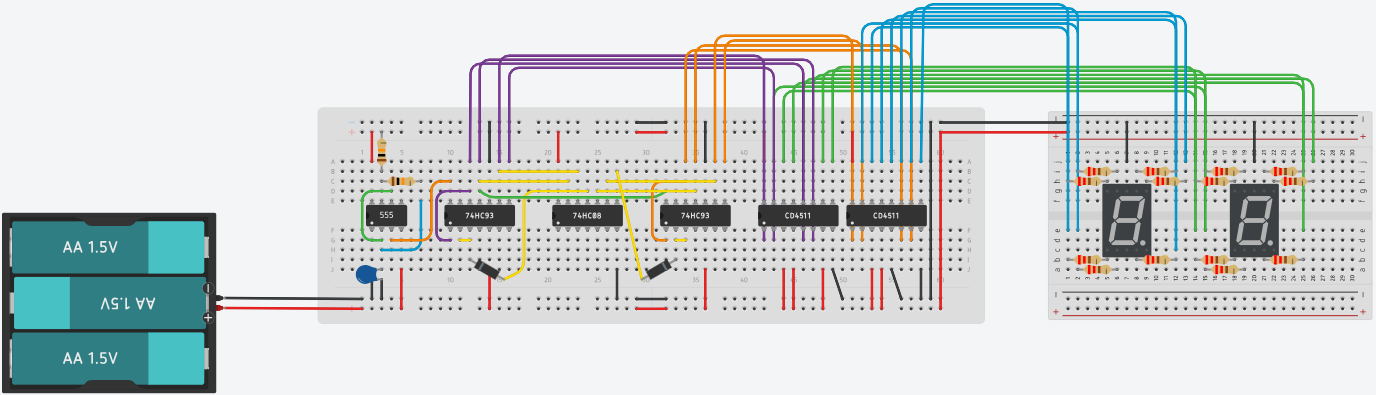
\includegraphics[width=1\linewidth]{images/image-4}
  \end{figure}
  \begin{center}
    Рисунок 4 – Схема сборки на макетной плате
  \end{center}

  \begin{figure}[h]
    \centering
    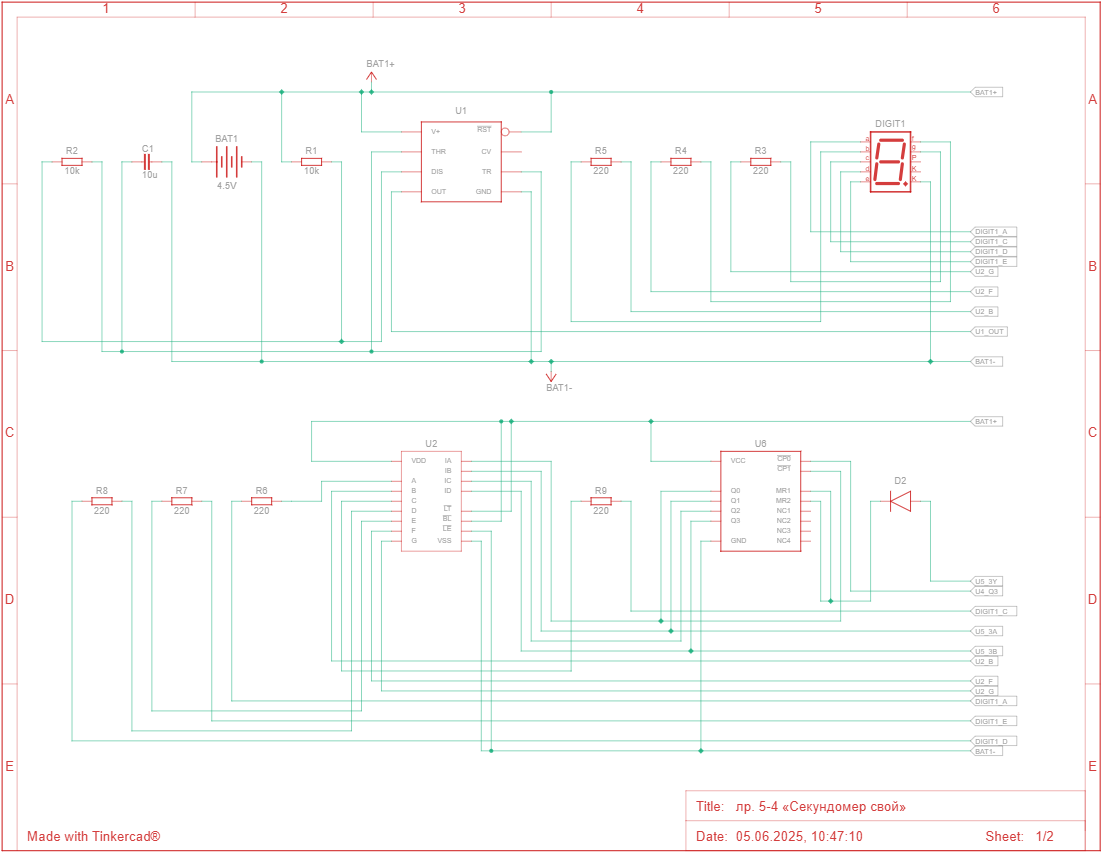
\includegraphics[width=0.72\linewidth]{images/image-5}
  \end{figure}
  \begin{center}
    Рисунок 5 – Принципиальная схема
  \end{center}

  \pagebreak

  \begin{figure}[h]
    \centering
    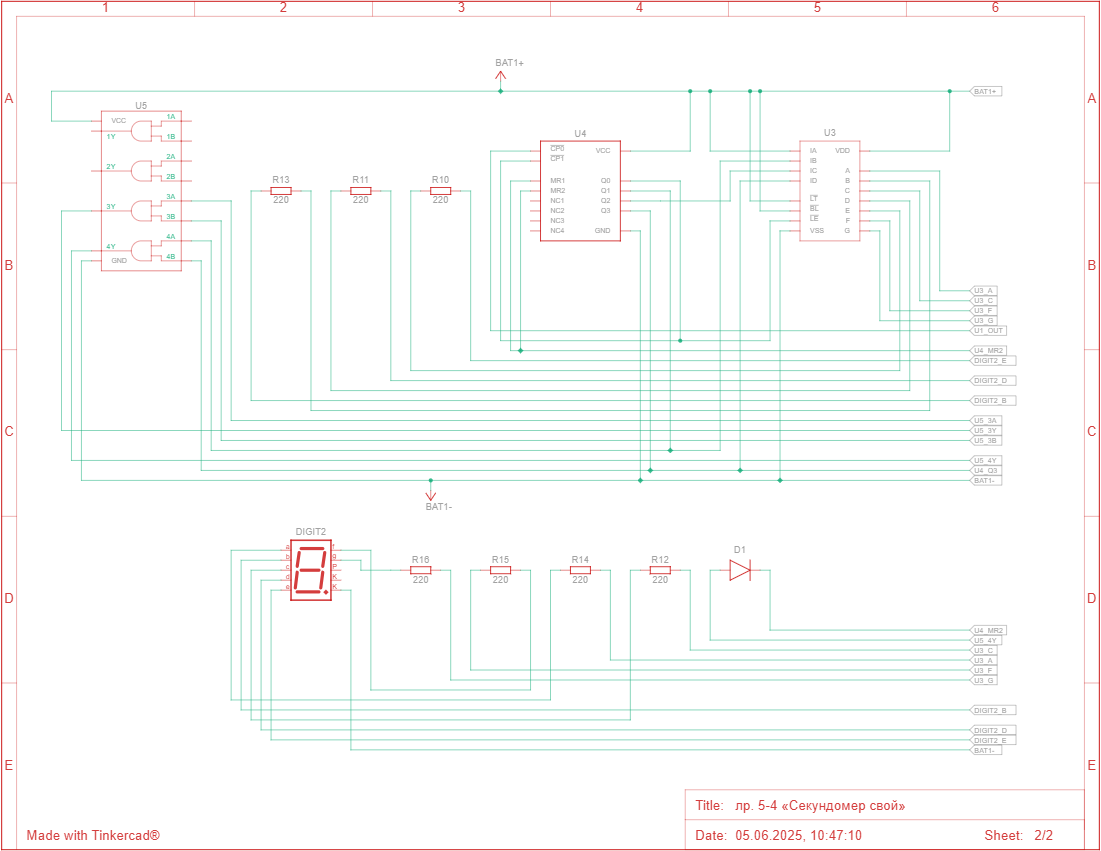
\includegraphics[width=0.72\linewidth]{images/image-6}
  \end{figure}
  \begin{center}
    Рисунок 6 – Принципиальная схема
  \end{center}

  \section*{\hspace{12.5mm}Вывод}
  В ходе лабораторной работы выполнены сборки без программирования, используя микросхемы стандартной логики.
 
\end{document}